\section{The Line: degree=1}
\label{sec.line}

\begin{figure}
  \centering
  %% derived from https://tex.stackexchange.com/questions/357538/graph-of-a-parabola-on-pgfplots
%% Thanks to Stefan Pinnow
%%     https://tex.stackexchange.com/users/95441/stefan-pinnow

\begin{figure}
  \centering
  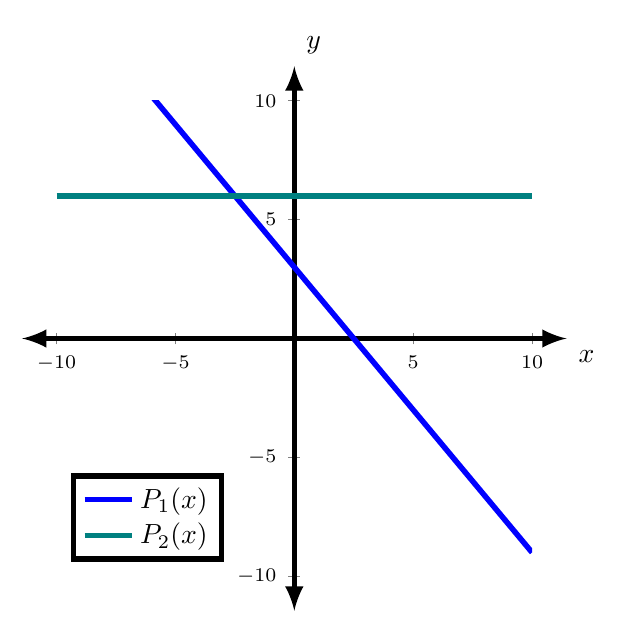
\begin{tikzpicture}
    \begin{axis}[
        legend pos=south west,
        samples=51,
        smooth,
        domain=-10:10,
        line width=2pt,
        width=3in,
        height=3in,
        axis lines=middle,
        xmin=-10,
        xmax=10,
        ymin=-10,
        ymax=10,
        scaled ticks=false,
        ticklabel style={font=\scriptsize},
        xlabel=$x$,
        ylabel=$y$,
        axis line style={
          latex-latex,
          shorten >=-12.5pt,
          shorten <=-12.5pt,
        },
        xlabel style={at={(ticklabel* cs:1)}, xshift=12.5pt, anchor=north west},
        ylabel style={at={(ticklabel* cs:1)}, yshift=12.5pt, anchor=south west},
      ]
      \addplot[color=blue] {-1.2*x + 3};
      \addlegendentry{\(P_1(x)\)}
      \addplot[color=teal] {6};
      \addlegendentry{\(P_2(x)\)}
    \end{axis}
  \end{tikzpicture}
  \caption{Line: $y = P(x) = -1.2*x + 3$}
  \label{fig.line}
\end{figure}

  \caption{Line: $y = P(x) = -1.2*x + 3$}
  \label{fig.line}
\end{figure}


\subsection{Objectives}
The assignment in this section is:
\begin{enumerate}
\item Complete the file \code{src/line.py} by writing a Python
  function which computes and returns the x-intercept of a line whose
  equation is ${y=a x + b}$.
\item You'll need to replace all occurances of \code{raise NotImplementedError()}
  with correct python code which passes the tests.

\item Test the function in GitHub Codespaces by running the file\\
  \code{test/test\_line.py}.
\end{enumerate}

\subsection{Overview}


A polynomial of degree 1 is a function $P(x)=a x + b$ whose graph is a line.   If $a=0$ the
line is horizontal an crosses the y-axis at $y=b$; thus if $b\neq 0$ then $P(x)\neq 0$.
So if $a=0$ we will assume that $P(x)$ has no root.   

\subsection{The Math}


Figure~\ref{fig.line} shows the graphs of two polynomials of degree 1.

\begin{align*}
  P_1(x) &= -1.2 x + 3\\
  P_2(x) &= 0 x + 6
\end{align*}

The line representing $P_1(x)$ has an x-intercept computed as in Example~\ref{ex.line}.


\begin{example}{Computing x-intercept of a line}{line}
  \begin{align*}
  P_1(x) &= a x + b \\
  0  &= -1.2 x + 3\\
  x &= \frac{3}{1.2} = 2.5
  \end{align*}
\end{example}

We see in Figure~\ref{fig.line} that if the coefficient of $x$ is 0, then the
line is horizontal and has no x-intercept. $P_2(x)$ is an example where $a=0$.
If the horizontal line $P_2(x)$is coincident
with the x-axis, \ie, if $a=0$ and $b=0$, then there is no unique x-intercept.





If $a\neq 0$,  then we have a line as shown in Figure~\ref{fig.line}.  We can
solve for the x-intercept by setting y to 0 and solving for x.
\begin{align*}
  y &= a x + b\\
  0 &= a x + b\\
  -b &= a x\\
  \frac{-b}{a} &= x
\end{align*}



\subsection{The Programming}


\begin{listing}{Function declaration to find x-intercept of a line.}{code.line}
\begin{minipage}[c]{0.95\textwidth}\begin{lstlisting}
def find_x_intercept(a,b):
    if a == 0:
        # CHALLENGE: student must complete the implementation.
        raise NotImplementedError()

    else:
        # CHALLENGE: student must complete the implementation.
        raise NotImplementedError()
\end{lstlisting}\end{minipage}\end{listing}


\begin{enumerate}

\item Open the file \code{src/line.py} in your web-based editor (GitHub Codespaces).
  You will develop the code in this file.

\item Find the occurances of \code{raise NotImplementedError()}.  This is the code that you must replace with working Python code.

\item You should update the code in the file \code{src/line.py} so that if
$a$ is 0, then the function returns an empty list and otherwise
  returns a list of the value~$\frac{-b}{a}$.

\item You must figure out how
to write that in the Python language.  \Ie, you must figure out how to
divde two numbers in Python and how to create a list, empty and
otherwise.


\item Test your code by running the pre-defined tests in \code{tests/test\_line.py}.

\item Look at the proposed solution in \code{solutions/line.py}.  It is not necessary that your code match exactly.

\end{enumerate}
